%%%%%
% ch5 %
%%%%%

\chapter{Forced and natural convection}
\section{Conduction and convection}
	\begin{wrapfigure}[10]{l}{4cm}
	\vspace{-5mm}
	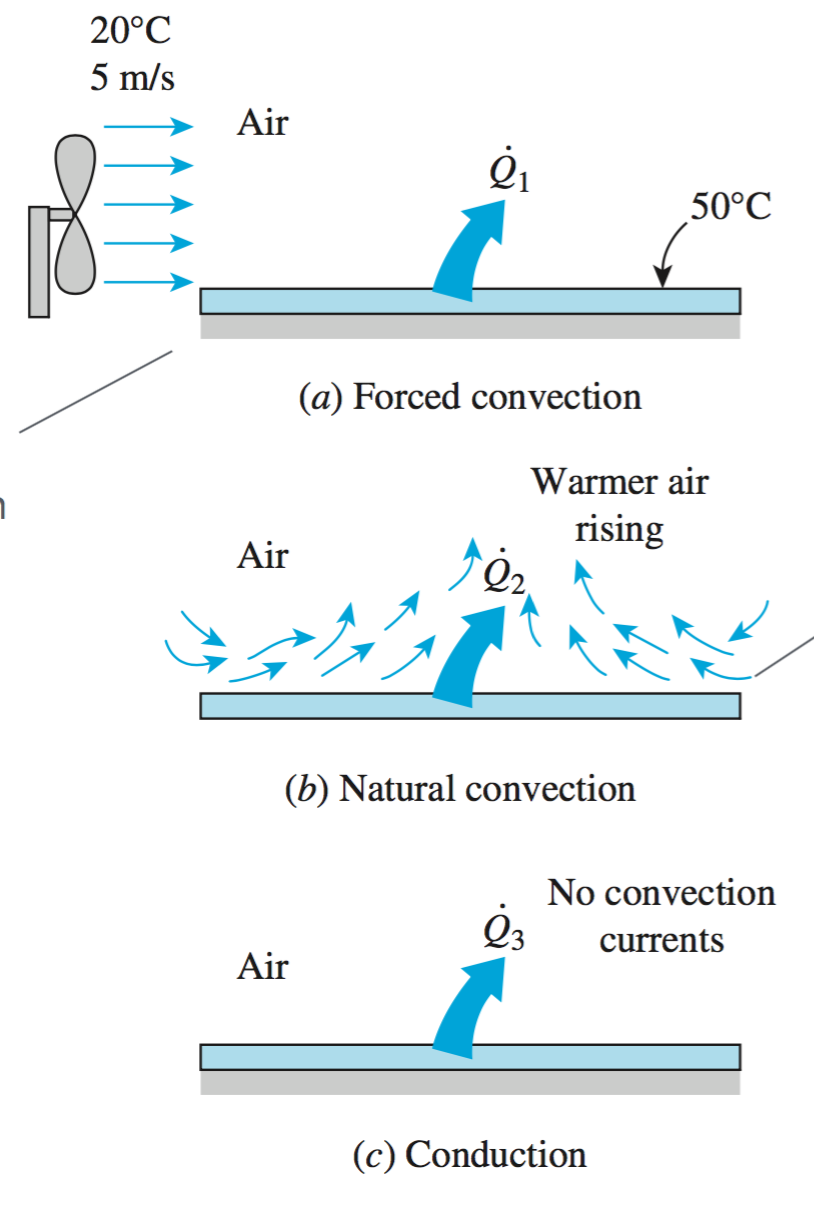
\includegraphics[scale=0.25]{ch5/1}
	\end{wrapfigure}	
	Heat transfer through a solid is always conduction, the molecules position are relatively fixed. Heat transfer in a liquid or gas is convection if there is a \textbf{bulk} fluid motion and is conduction when there isn't. Conduction in a fluid is the limiting case of convection where the fluid is \textbf{quiescient}\footnote{Au repos}.  \\
	Convection is complicated due to the fact that it involves fluid motion as well as conduction. Fluid motion \textbf{enhances}\footnote{Améliore} fluid motion, it brings the cooler and warmer part of fluid into contact, increasing the rate of heat transfer. \\
	Natural convection is caused by a density gradient. 

\section{Macroscopic energy balance}
	\begin{wrapfigure}[6]{r}{5cm}
	\vspace{-5mm}
	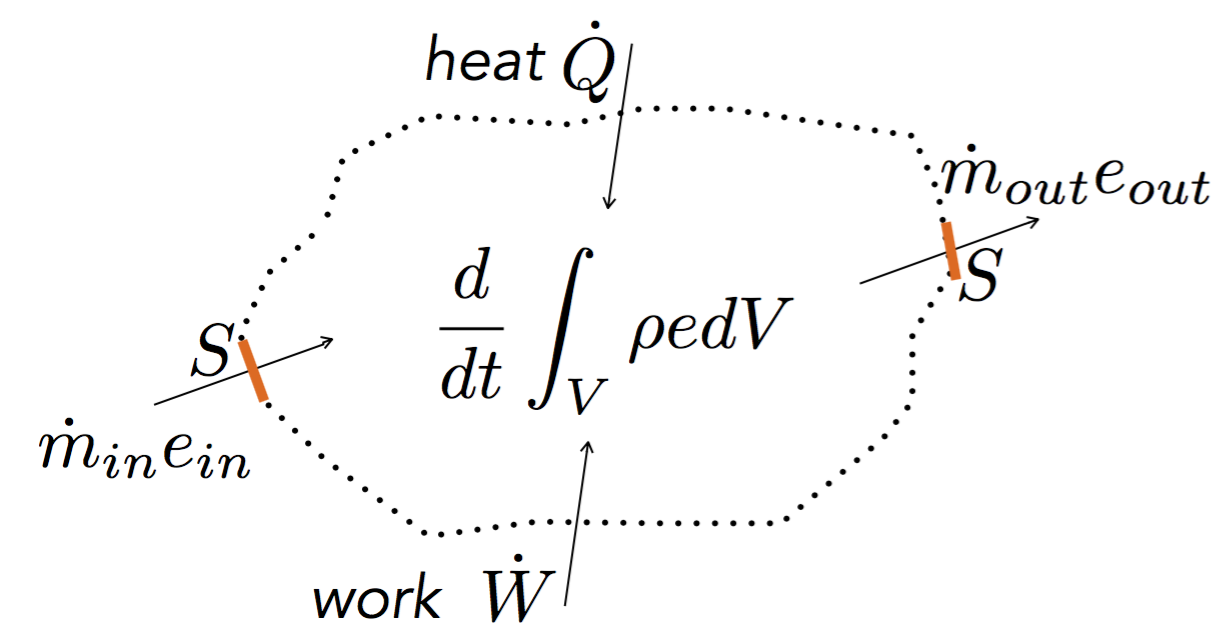
\includegraphics[scale=0.25]{ch5/2}
	\end{wrapfigure}	
	Let's consider a control volume and let's apply an energy balance, using $e = u + \frac{v^2}{2} + gz$ where the first term is the internal energy, the second the kinetic energy and the last the potential energy 
	\begin{equation}
		\frac{d}{dt}\int _V \rho e \, dV = (\rho v e S)_{in} - (\rho v e S)_{out} + \dot{W} + \dot{Q}
	\end{equation}
	Where the work can be decomposed in a \textbf{boundary} and a \textbf{useful} work and the heat is given by
	\begin{equation}
		\dot{W} = \dot{W}_f + \dot{W}_p = pvS + \dot{m}w_p = \dot{m}\left( \frac{p}{\rho}+w_p \right) \qquad and \qquad \dot{Q} = \dot{m} q
	\end{equation}		 
	The transient form is given by 
	\begin{equation}
		\frac{d}{dt}\int _V \rho e \, dV = - \Delta (\frac{1}{2}\rho v^3S) - g \Delta (\rho v z S) - \Delta (pvS) - \Delta (\dot{m}u) + \dot{m}w_p + \dot{m}q
	\end{equation}
	The steady form 
	\begin{equation}
		0 = \Delta \left( \frac{1}{2}v^2 + gz + u + \frac{p}{\rho} \right) - q - w_p 
		\label{eq:5.4}
	\end{equation}
	
	\subsection{Relation with the generalized Bernouilli equation}
		Let's take the steady form of the energy balance for a finite transformation \autoref{eq:5.4} and let's convert it for an infinitesimal transformation 
		\begin{equation}
			0 = - \left( \frac{1}{2}dv^2 + g dz + d\left(\frac{p}{\rho}\right) \right) + (\delta q - du) + dw_p
			\label{eq:5.5}
		\end{equation}
		Let's remind (see \emph{Chimie-Physique}) that the \textbf{Gibbs equation} (corresponding to elemental working change) and the \textbf{second principle} of thermdynamics are given by the expressions
		\begin{equation}
			du = Tds - pdV \qquad and \qquad Tds - \delta q= dh_f \geq 0
		\end{equation}
		Combining the two equations around $Tds$
		\begin{equation}
			\delta q - du = -dh_f + pdV
		\end{equation}
		and replacing in \autoref{eq:5.5}, we obtain the \textbf{generalized Bernouilli equation}
		\begin{equation}
			\frac{1}{2}dv^2 + g dz + \frac{dp}{\rho} = w_p - dh_f \qquad
			 \underset{\rho = cst}{\longrightarrow} \qquad 
			 \frac{1}{2}\Delta v^2 + g \Delta z + \frac{\Delta p}{\rho} = w_p - h_f 
		\end{equation}
		
	\subsection{Simplification in case of heat exchange}
		When we analize heat exchange processses, we assume that we can also consider the variation of enthalpy. We can so rewrite the expression and make appear the heat flux in function of the difference of enthalpy in the streams. So we have 
		\begin{equation}
			u + \frac{p}{\rho} = u + pv = h \qquad and \qquad \underbrace{\Delta h = \int _{T_0}^T c_p \, dT}_{Gas} \qquad \underbrace{\Delta h = c\Delta T}_{Liquid}
		\end{equation}
		We assume that thermal power is much higher than the power for pumps and compressors and that the enthalpy change is much higher than the kinetic and potential energy variation. Applying all that to equation \autoref{eq:5.4}, we have
		\begin{equation}
			\dot{Q} = \dot{m}\Delta h = \Delta \dot{H}
		\end{equation}
		
\section{The heat transfer coefficient}
	The rate of convection $\dot{Q}$ is proportional to the temperature difference. 
	\begin{equation}
		\dot{Q} = h S(T_p - T_f)
	\end{equation}		
	\begin{wrapfigure}[3]{l}{4cm}
	\vspace{-15mm}
	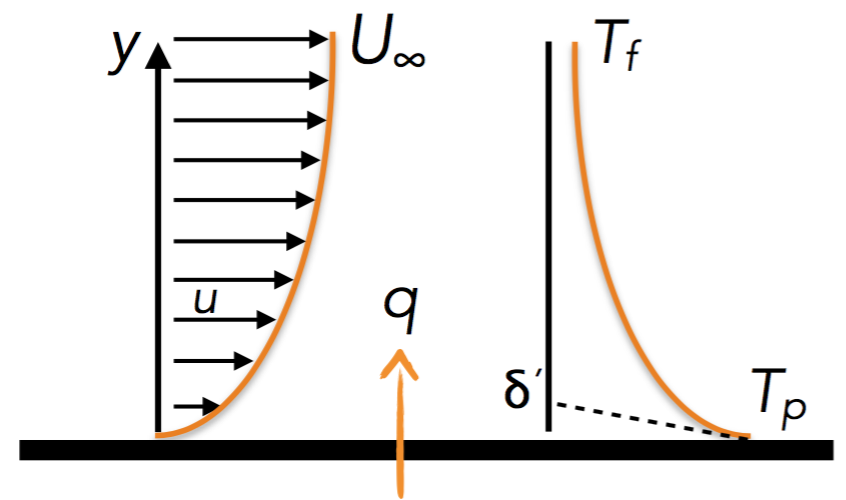
\includegraphics[scale=0.25]{ch5/3}
	\end{wrapfigure}	
	$h$ here is not the enthalpy but the \textbf{heat transfer coefficient}. Let’s give a sens. Imagine that you have a fluid flow and it is approaching a solid. The heat transfer from solid surface to the fluid layer is by pure conduction, since the fluid layer beys the no-slip conditions. Now if you have $T_p$ miner than $T_f$ we have that type of schéma. The heat is then convected 
 

